\documentclass{hhu-thesis-bachelor}
%% 更改数学字体设置,Latin Modern Math 默认的有点细,可选用下列宏包
% \usepackage[bold-style=ISO]{unicode-math}
\usepackage{lipsum}

%% 本科论文规定不允许有空页,因此将空页替换掉
\let\cleardoublepage\clearpage

\begin{document}

%%
%% 基本信息设定(一定要改这里)
%%

% 此处填写你的学号
\studentnumber{1812100019}
% 此处填写你的中文论文标题
\title{分布式智能监控终端\\与传感信息融合系统设计及实现}
% 此处填写你的中文姓名
\author{张晓明}
% 此处填写你的年级,如:2018级
\grade{2018级}
% 此处填写指导教师的中文名
\tutor{毛明禾}
% 此处填写专业的中文名
\major{电子信息工程}
% 此处填写日期,如:2022年5月
\thesisdate{2022年5月}
% 此处填写中文地点,如:中~~国~~$\cdot$~~南~~京,将城市名改成所在的城市即可
\location{中~~国~~$\cdot$~~南~~京}

% 此处填写英文论文标题
\englishtitle{Design and implementation of distributed smart monitoring terminal and sensor information fusion system}
% 此处填写英文学院名
\englishcollege{Computer and information}
% 此处填写英文专业名
\englishmajor{Electronics and Information Engineering}
% 此处填写你的英文姓名
\englishauthor{Xiaoming Zhang}
% 此处填写指导教师的英文名
\englishtutor{Dr. Minghe Mao}
% 此处填写英文地点,如:Nanjing,  P.R.China
\englishlocate{Nanjing,  P.R.China}

%%
%% 生成封面和声明页
%%

%% 生成中文封面
\makecover
%% 生成英文封面
\makeencover
%% 生成声明页
\makedeclare

%%
%% 前置部分
%%

\frontmatter
%% 摘要
%% This is file 'abstract.tex'
%% It is included by hhuthesis-example.tex for hhuthesis.
%%
%% Copyright(C) 2020-2021, Wenhan Cao
%% College of Water Conservancy and Hydropower Engineering, Hohai University.
%%
%% Version:v2.0.0
%% Last update: April 7th, 2021.
%%
%% Home Page of the Project: https://github.com/caowenhan/thesis
%%
%% This file may be distributed and / or modified under the conditions of the
%% LaTeX Project Public License, either version 1.3c of this license or (at your
%% option) any later version. The latest version of this license is in:
%%
%% http://www.latex-project.org/lppl.txt
%%
%% and version 1.3c or later is part of all distributions of LaTeX version
%% 2008/05/04 or later.
%%

\begin{abstract}
	本文首次提出并建立了诸如组合单元水力计算正问题、组合单元水质正问题、水量模型参数反问题、水质边界条件及污染源项反问题等系列成果。主要研究内容如下:
\begin{enumerate}
	\item[(1)] 组合单元水力计算正问题。
	\item[(2)] 组合单元水质正问题。
\end{enumerate}


\keywords{河网;力特征;水质特性;污染面;联合解法}
\end{abstract}

\begin{enabstract}
	This paper makes more systematic and deeper studies on numerical simulations of hydraulics and water quality features of river networks. As a result, a series of achievements such as combined cells model of hydraulics, combined cells model of water quality, roughness parameter reverse problem, waste load reverse problem and simulation of hydraulics boundary condition have been put forward for the first time. The details are as follows:

\begin{enumerate}
\item[(1)] combined cells model of hydraulics.
\item[(2)] combined cells model of water quality.
\end{enumerate}  
 
\enkeywords{River network; Force characteristics; Water quality characteristics; Pollution surface; Joint solution}

\end{enabstract}

%% 符号对照表,可选,如不用可注释掉
% %% This is file 'denotation.tex'
%% It is included by hhuthesis-example.tex for hhuthesis.
%%
%% Copyright(C) 2020-2021, Wenhan Cao
%% College of Water Conservancy and Hydropower Engineering, Hohai University.
%%
%% Version:v2.0.0
%% Last update: April 7th, 2021.
%%
%% Home Page of the Project: https://github.com/caowenhan/thesis
%%
%% This file may be distributed and / or modified under the conditions of the
%% LaTeX Project Public License, either version 1.3c of this license or (at your
%% option) any later version. The latest version of this license is in:
%%
%% http://www.latex-project.org/lppl.txt
%%
%% and version 1.3c or later is part of all distributions of LaTeX version
%% 2008/05/04 or later.
%%

\begin{denotation}
	
\item[\LaTeX] 一个很棒的排版系统
\item[\LaTeXe] 一个很棒的排版系统的最新稳定版
\item[\XeTeX] \LaTeX{}的好兄弟,事实上他有很多个兄弟,但是这个兄弟对各种语言的支持能力都很强
\item[ctex] 成套的中文\LaTeX{}解决方案
\item[\ce{CaCO3}] 碳酸钙
\item[$ e^{\pi{}i}+1=0$] 集自然界五大常数一体的最美方程,欧拉公式

\end{denotation}

%% 加入目录
\tableofcontents
%% 加入图、表索引(同时取消图表索引中章之间的垂直间隔,不需要可以注释)
\let\origaddvspace\addvspace
\renewcommand{\addvspace}[1]{}
\listoffigures
\listoftables
\renewcommand{\addvspace}[1]{\origaddvspace{#1}}

%%
%% 正文部分
%%

\mainmatter
%% 各章正文内容
%% 在这里引入你的各个章节哦!!!
%% This is file 'chapter1.tex'
%% It is included by hhuthesis-example.tex for hhuthesis.
%%
%% Copyright(C) 2020-2021, Wenhan Cao
%% College of Water Conservancy and Hydropower Engineering, Hohai University.
%%
%% Version:v2.0.0
%% Last update: April 7th, 2021.
%%
%% Home Page of the Project: https://github.com/caowenhan/thesis
%%
%% This file may be distributed and / or modified under the conditions of the
%% LaTeX Project Public License, either version 1.3c of this license or (at your
%% option) any later version. The latest version of this license is in:
%%
%% http://www.latex-project.org/lppl.txt
%%
%% and version 1.3c or later is part of all distributions of LaTeX version
%% 2008/05/04 or later.
%%
\chapter{绪论}
\label{chap:introduction}
\section{河网水力及水质特性数值模拟研究的意义}
\label{sec:meaning}

随着近年来工农业生产的迅猛发展,在河网地区,水资源的供给与需求、环境质量与经济发展这两对矛盾日益突出\cite{tongjiju1997}。环境质量的日趋恶化将愈来愈威胁着区域经济的健康发展,环境治理已成为亟待解决的重大课题\cite{zhengxiaoyu1994}。……\par
……\par
……\par

\section{河网水力及水质特性数值模拟研究综述}

\subsection{水力模拟研究综述}
河网非恒定流的水力特性模拟研究时水利、航运及环保等部门经常进行的工作\cite{liyitian1997}。由于河网区域范围广大,因此只能采用数值方法进行模拟。……\par
……\par
……

\subsubsection{水力数值模拟方法研究}
按控制方程及对河网处理方式的不同,数值模拟方法可分为两大类:第一类为人们所熟知的圣维南方程组求解法,第二类为由法国Jean A.Cunge提出的所谓“组合单元法”\cite{halts1996}。……\par
……\par
……\par
……

\section{技术路线和研究内容}
作为本文核心部分,作者深入系统地研究了平原河网水量水质数值模拟的正反两方面的问题。首次提出用“组合单元法”数值模拟平原河网水力水质特性,分别给出了水量、水质数值模拟的正问题的稀疏矩阵求解方程式及单元分组求解方程式,为平原河网水量水质数值计算开辟了一条新的途径。在正问题的基础上,首次提出:生成基本解,用基本解构造水质边界条件反问题及源项反问题,并采用优化方法中诸如简约梯度法等方法以及遗传算法等方法分别对无约束及有约束的非线性规划问题进行求解。……\par
……\par
……\par
本文的主要研究内容见图\ref{fig:maincontents}。

\begin{figure}[H]
	\centering
	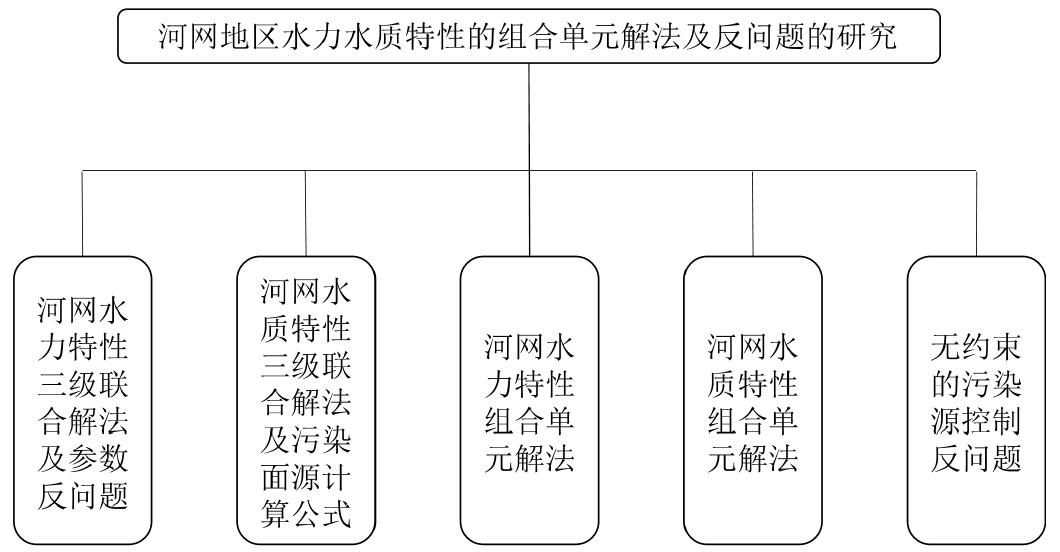
\includegraphics[width=0.75\textwidth]{figure1.jpg}
	\caption{论文的主要研究内容} \label{fig:maincontents}
	%硕士论文、本科毕业论文不使用双语图表标题,可使用命令\caption{}替代\caption{}
\end{figure}


%% This is file 'chapter2.tex'
%% It is included by hhuthesis-example.tex for hhuthesis.
%%
%% Copyright(C) 2020-2021, Wenhan Cao
%% College of Water Conservancy and Hydropower Engineering, Hohai University.
%%
%% Version:v2.0.0
%% Last update: April 7th, 2021.
%%
%% Home Page of the Project: https://github.com/caowenhan/thesis
%%
%% This file may be distributed and / or modified under the conditions of the
%% LaTeX Project Public License, either version 1.3c of this license or (at your
%% option) any later version. The latest version of this license is in:
%%
%% http://www.latex-project.org/lppl.txt
%%
%% and version 1.3c or later is part of all distributions of LaTeX version
%% 2008/05/04 or later.
%%
\chapter{河网水力特性三级联合解法及参数反问题}
\label{chap:inverseproblem}
\section{概述}
河网的非恒定流计算通常采用三级联合解法,此方法可归结为一维圣维南方程组的求解问题,即对组成河网的每条河道采用有限差分的隐式格式离散圣维南方程组,得到线性差分方程组。……\par
……
\section{河道控制方程}
描述明渠一维非恒定流的基本方程为一维Saint-Venant 方程组:
\begin{equation}
	\frac{\partial Q}{\partial x}+B_{W}\frac{\partial Z}{\partial t}=q
\end{equation}
\begin{equation}
	\frac{\partial Q}{\partial t}+2u\frac{\partial Q}{\partial x}+(gA-Bu^{2})\frac{\partial Z}{\partial x}-u^{2}\frac{\partial A}{\partial x}+g\frac{n^{2} |u|Q}{R^{4/3}}=0
\end{equation}
\noindent 式中,$t$为时间坐标;$x$为空间坐标;……\par
……\par
……

\section{边界条件}
……\par
……

\section{方程的求解}
……\par
……

\section{参数反问题}
……\par
……

\section{算例分析}
为了验证上述计算方法的可靠性,通常借用正问题的解来构造反问题。即先进行正问题计算,用其结果验证反问题的解。\par
……\par
……\par
计算结果见表\ref{tab:parameter}。

\begin{table}[H]\small	%\small用于控制表格内字体大小为5号字
	\centering
	\bicaption{参数理论值与最优解}{Theoretiacal value and optimal solution of the parameter} \label{tab:parameter}
	\begin{tabular*}{0.75\textwidth}{@{\extracolsep{\fill}}cccc}
		\toprule
		\multicolumn{1}{l}{} & b1     & b2     & b3     \\\midrule
		理论解                  & 22     & 18     & 16     \\
		最优解1                 & 21.986 & 18.048 & 15.997 \\
		最优解2                 & 21.997 & 18.011 & 15.999 \\ \bottomrule
	\end{tabular*}%
\end{table}


……\par
……
\section{本章小结}
本章采用平原河网三级联合解法水量模型模拟河网的水力要素,建立了平原河网
水量模型,对位于长江下游的南通河网进行了模拟运算。\par
……\par
……


%% 参考文献样式设定
\bibliographystyle{hhuthesis-numeric}% 顺序编码式

%% 参考文献,10号字,使用 BibTeX,包含参考文献文件.bib
%% 如果新创建了bib文件,记得要在这里引用哦!!!
\bibliography{reference/chap1}

%%
%% 后置部分
%% 

%% (其后部分无编号)
\backmatter
%% 致谢
%% This is file 'acknowledgement.tex'
%% It is included by hhuthesis-example.tex for hhuthesis.
%%
%% Copyright(C) 2020-2021, Wenhan Cao
%% College of Water Conservancy and Hydropower Engineering, Hohai University.
%%
%% Version:v2.0.0
%% Last update: April 7th, 2021.
%%
%% Home Page of the Project: https://github.com/caowenhan/thesis
%%
%% This file may be distributed and / or modified under the conditions of the
%% LaTeX Project Public License, either version 1.3c of this license or (at your
%% option) any later version. The latest version of this license is in:
%%
%% http://www.latex-project.org/lppl.txt
%%
%% and version 1.3c or later is part of all distributions of LaTeX version
%% 2008/05/04 or later.
%%

\begin{acknowledgement}

本文是在导师张长江教授的精心指导下完成的。值此论文完稿之际,谨向导师及所有帮助过我的各位表示诚挚的谢意。\par
……\par
……\par
还要特别感谢hhu-thesis-bachelor节省了论文排版的时间。
\vspace{5cm}
\begin{flushright}
	作者:韩中国\\
	2016年12月于南京
\end{flushright}

\end{acknowledgement}

\end{document}